\documentclass{article}
\usepackage{import}
\usepackage[ruled]{algorithm2e}
\usepackage[shortlabels]{enumitem}
\usepackage{hyperref}
\usepackage{minted}
\usepackage{subcaption}

\hypersetup{
    colorlinks=true,
    linkcolor=blue,
    filecolor=magenta,      
    urlcolor=cyan,
    pdftitle={Overleaf Example},
    pdfpagemode=FullScreen,
    }
\subimport*{}{macro}

\setlength\parindent{0px}

\begin{document}
\setcounter{problem}{0}
\title{Homework \#4}
\author{
    \normalsize{AA 597: Networked Dynamics Systems}\\
    \normalsize{Prof. Mehran Mesbahi}\\
    \normalsize{Due: Feb 9, 2024 11:59pm}\\
    \normalsize{Soowhan Yi}
}
\date{{}}
\maketitle

All the codes are available at the end of the documents or here.
\url{https://github.com/SoowhanYi94/ME597}
\begin{problem}2.15
    Let $G = (V, E)$ be a graph, and let $uv \notin E$ for some $u, v \in V$. Show that
    \begin{align*}
        \lambda_2 (G) \leq \lambda_2(G+e) \leq \lambda_2 + 2
    \end{align*}
    where $G + e$ is the graph $(V, E \cup {e})$.

    According to Courant-Fischer theorem, $\min_{||x|| = 1} x^T A x = \lambda_1$ and $\min_{||x|| = 1, x\perp 1} x^T A x = \lambda_2$ where v is a eigenvector corresponding to $\lambda_1$, when A is symmetric. For some graph G, which has u and v as a vertex but (uv) is not a edge. Lets say that this (uv) edge is added to the graph. Then, the degree in u and v vertices are going to increase by 1, and adjacentcy matrix, A, would have extra 1s in $A_{uv}$ and $A_{vu}$. Therefore, where $G + e = G^{'}$, 
    \begin{align*}
        &x^T L(G) x = \sumi{1}{n} D_{ii} x_i^2 - \sumi{1}{n} \sumj{1}{n} A_{ij}x_i x_j 
        , \quad \textrm{and} \quad \space x^T L(G^{'}) x = \sumi{1}{n} D^{'}_{ii} x_i^2 - \sumi{1}{n} \sumj{1}{n} A^{'}_{ij}x_i x_j \\
        &\min_{||x|| = 1, x\perp 1} x^T L(G) x = \lambda_2,\quad \textrm{and} \quad \min_{||x|| = 1, x\perp 1} x^T L(G^{'}) x = \lambda_2^{'}
    \end{align*},
    \begin{align*}
        x^T L(G^{'}) x &= \sumi{1}{n} D^{'}_{ii} x_i^2 - \sumi{1}{n} \sumj{1}{n} A^{'}_{ij}x_i x_j \\
        &=(\sumi{1}{n} D_{ii} x_i^2 - \sumi{1}{n} \sumj{1}{n} A_{ij}x_i x_j) + x_u x_u + x_v x_v - x_u x_v - x_v x_u\\
        &=   x^T L(G) x + (x_u - x_v)^2\\
        \therefore  \min_{||x|| = 1, x\perp 1} x^T L(G^{'}) x &=  \min_{||x|| = 1, x\perp 1} (x^T L(G) x  + (x_u - x_v)^2) = \lambda_2(G^{'})  \\
        \min_{||x|| = 1, x\perp 1} (x^T L(G) x  + (x_u - x_v)^2) &\geq \lambda_2(G) + \min_{||x|| = 1, x\perp 1} (x_u - x_v)^2   \geq \lambda_2(G)
    \end{align*}
    Also, $||x|| = 1$. Therefore $x_1^2 + x_2^2 + \cdots +  x_u ^2 + \cdots +  x_v^2 + \cdots x_n^2 = 1 $. Lets say, hypothetically, $ x_1 = x_2 = \cdots = x_n = 0$, but $x_u \neq 0$, and $x_v \neq 0$. Since the minimum value of $x_u x_v$, under $x_u^2 + x_v^2 = 1$, is $-\frac{1}{2}$(this can be calulated with use of lagrangian. $L(x_u, x_v, \alpha) = x_u x_v + \alpha (1 - x_u^2 - x_v^2$), then, 
    \begin{align*}
        &x_u^2 + x_v^2 = 1\\
        &L(x_u, x_v, \alpha) = x_u x_v + \alpha (1 - x_u^2 - x_v^2)\\
        &\frac{\delta L}{\delta x_u} = x_v - 2 \alpha (x_u) = 0, \quad
        \frac{\delta L}{\delta x_v} = x_v - 2 \alpha (x_v) = 0 \quad
        \frac{\delta L}{\delta \alpha} = 1 - x_u^2 - x_v^2 = 0\\
        \therefore & \min{x_u x_v}  = -\frac{1}{2}. (\because x_u = \pm \frac{1}{\sqrt{2}}, x_v = \mp \frac{1}{\sqrt{2}})\\
        &(x_u - x_v)^2  = (1 - 2 x_u x_v) = 1 + 1 = 2 
    \end{align*}
    Therefore maximum value that $(x_u - x_v)^2$ can be is 2. 
    \begin{align*}
        \lambda_2 (G) \leq \lambda_2(G+e) \leq \lambda_2 + 2
    \end{align*}
\end{problem}
\begin{problem}3.3
    The reverse of D is a digraph where all directed edges of D have been reversed. A disoriented digraph is the graph obtained by replacing the directed edges of the digraph with undirected ones. Prove or disprove:
    \begin{enumerate}
        \item The digraph D is strongly connected if and only if its reverse is strongly connected.
        
            By definition, strongly connected means that every pair of vertices has at least one directed path. This means that every node is reachable with random initial conditions. Lets say,for strongly connected $G = (V, E)$, $u,v \in V$, and there exists a directed path from u to v and v to u. If we were to reverse all those directions, then there would still exist a directed path from v to u and u to v, respectively. Therefore the reverse of strongly connected digraph D would also have at least one directed path for every pair of vertices. Therefore reverse of strongly connected D is also strongly connected. 
            If the reverse is not strongly connected, then that means their is some directed path missing in some pair of vertices, and therefore original graph would not be strongly connected with some missing directed path as there is no edge. Therefore the digraph D is strongly connected if and only if its reverse is strongly connected. So the statement is true
        \item A digraph contains a rooted out-branching if and only if its reverse digraph contains one.
        \begin{figure*}[!h]
            \centering
            \begin{subfigure}{0.35\textwidth}
                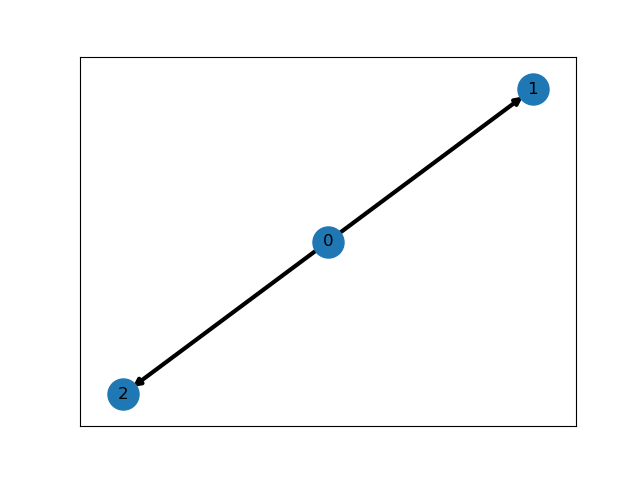
\includegraphics[width=\textwidth]{./img/p2_1.png}
                \caption{Directed graph with 3 nodes}
            \end{subfigure}
            \begin{subfigure}{0.35\textwidth}
                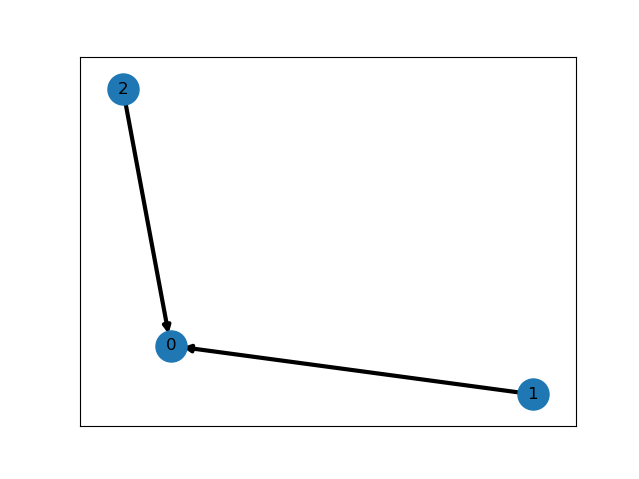
\includegraphics[width=\textwidth]{./img/p2_2.png}
                \caption{Reversed directed graph}
            \end{subfigure}
        \end{figure*}
        
        As we can see from above, a digraph with 3 nodes and rooted out-branching at node 0. However the reversed version of the digraph does not contain rooted out-branching. So the statement is false.
        \item If the disoriented graph of D is connected, then either the digraph or its reverse contain a rooted out-branching.
        \begin{figure*}[!h]
            \centering
            \begin{subfigure}{0.3\textwidth}
                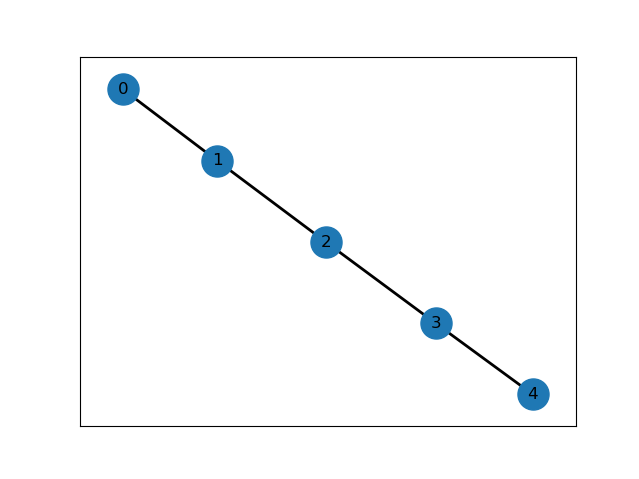
\includegraphics[width=\textwidth]{./img/p2_3.png}
                \caption{Undirected graph with 5 nodes}
            \end{subfigure}
            \begin{subfigure}{0.3\textwidth}
                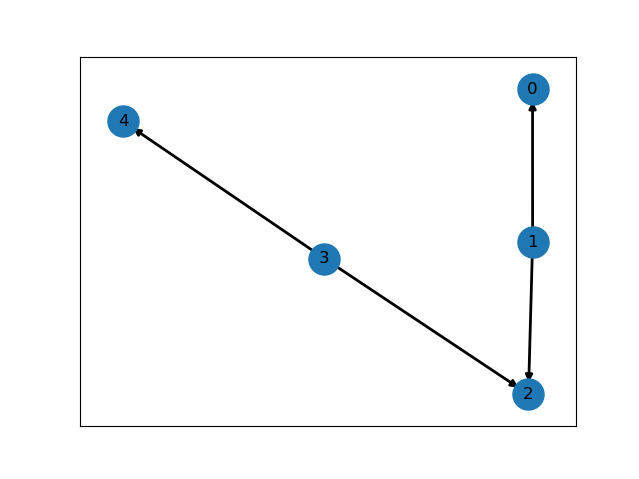
\includegraphics[width=\textwidth]{./img/p2_4.png}
                \caption{Directed graph with 5 nodes}
            \end{subfigure}
            \begin{subfigure}{0.3\textwidth}
                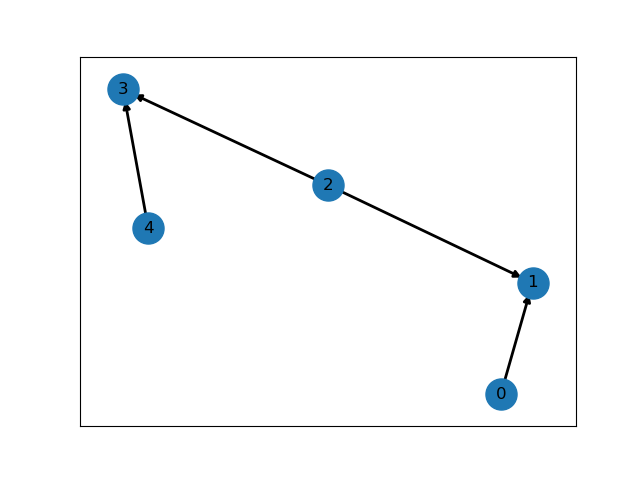
\includegraphics[width=\textwidth]{./img/p2_5.png}
                \caption{Reversed directed graph}
            \end{subfigure}
        \end{figure*}
        
        As we can see from above, the disoriented graph of D is connected. The second graph is the original graph. Here we do not see a single node that can reach every other nodes. There is no rooted out-branching in original digraph, with $[(1, 0), (1, 2), (3, 2), (3,4)] \in E$. Also we can see that the reverse do not have any node as rooted out-branching. Therefore the statement is false.  
        \item A digraph is balanced if and only if its reverse is balanced.
        
        The definition of balanced digraph is the directed graph that every nodes has same in-degree and out-degree, meaning if there is a directed edge towards or in to the nodes, then there exists a directed edge going away or out of the node. If a node has n edges coming in to the node, then there should be another n edges that goes out from the node. Even if the graph is reversed, there would still be same in-degree and out-degree as we started with same number of edges going in to the node and out from the node. Therefore the statement is true. If reversed was not balanced, the digraph would not be balanced. 
    \end{enumerate}
\end{problem}
\begin{problem} 4.8
    Consider n agents placed on the line at time t, with agent1 at position 2 $\Delta$, agent2 at position $\Delta$ and the remaining agents at the origin. An edge between agents exists if and only if $|x_i - x_j| \leq \Delta$. Compute where the agents will be at time $t + \delta t$ for some small $\delta t$, under the agreement protocol. In particular, for what values of n is the graph connected at time $t + \delta t$?

    Let $z(k) = x(k\delta t)$ and $k\delta t = \tau$. Then, 
    \begin{align*}
        &z(k + 1) = e^{-\delta t L(G)} z(k) = x((k+1)\delta t)=  x(k \delta t + \delta t)\\
        &=e^{-\delta t L(G)}  x(\tau) = x (\tau + \delta t)\\
        \therefore & x (\tau + \delta t) = e^{-\delta t L(G)}  x(\tau) = (e^{-\delta t L(G)} ) x(\tau) \text{ where } |x_i - x_j|\leq \Delta (\because \text{in order to stay connected})
    \end{align*}
    Now lets think about the $L(G)$. Since edges are formed when $|x_i - x_j| \leq \Delta$, every vertices are connected except for the very first vertex. The first vertex is only connected to the second one. This means that it forms a complete graph $K_{n-1}$ with the very first vertex only being connected to the second one. Therefore the degree matrix should be $D(G) = diag([1, n-1, n-2 \cdots , n-2])$ and $A(G)$ should have all ones except for the diagonal and the first row and column. The first row and column only has 1 at 2nd row in first colum and 2nd column in first row. Therefore, 
    \begin{align*}
        &-L(G) = \begin{bmatrix*}
            -1 & 1 & 0 & 0 & \cdots &0 \\
             1 & 1-n & 1 & 1 & \cdots & 1\\
             0 & 1 & 2-n & 1 & \cdots & 1 \\
             \vdots & \vdots & 1&2-n &1 \cdots &1\\
             0& 1&1&\cdots &1&2-n\\
        \end{bmatrix*}
    \end{align*}
    Lets use the provided initial conditions $[2\Delta, \Delta, 0, 0, 0, \cdots 0]$. Also for small enough $\delta t$, we can approximate $e^{-\delta t L(G)}$ as $I + \delta t L(G)$, with power series. So now we have, 
    \begin{align*}
        x (\tau + \delta t) &= e^{-\delta t L(G)}  x(\tau) =(I - \delta t L(G))x(\tau)\\
        &=x(\tau) - \delta t L(G) x(\tau)\\
        &= \begin{bmatrix*}
            2 \Delta \\
            \Delta\\
            0\\
            \vdots\\
            0
        \end{bmatrix*} + 
        \delta t \begin{bmatrix*}
            -1 & 1 & 0 & 0 & \cdots &0 \\
             1 & 1-n & 1 & 1 & \cdots & 1\\
             0 & 1 & 2-n & 1 & \cdots & 1 \\
             \vdots & \vdots & 1&2-n &1 \cdots &1\\
             0& 1&1&\cdots &1&2-n\\
        \end{bmatrix*} 
        \begin{bmatrix*}
            2 \Delta \\
            \Delta\\
            0\\
            \vdots\\
            0
        \end{bmatrix*} \\
        &= \begin{bmatrix*}
            2\Delta - \delta t \Delta\\
            \Delta +  \delta t (3-n)\Delta\\
            \Delta \delta t\\
            \vdots\\
            \Delta \delta t
        \end{bmatrix*}\\
        &\therefore 2\Delta - \delta t \Delta -(\Delta +  \delta t (3-n)\Delta) \leq \Delta \text{ to be connected}\\
        &\delta t (n-4) \leq 0
    \end{align*} 
    Therefore, for any small enough $\delta t$, n should be less than 4. 
\end{problem}
\newpage
\begin{problem}6.5
    If a team of robots is to drive in formation while avoiding obstacles as well as progressing toward a goal location, one can, for example,let the individual agent dynamics be given by
    \begin{align*}
        \dot x_i = F_{form} + F_{goal} + F_{obst}
    \end{align*}
    where $f_{form}$ is used to maintain formation. However, $F_{goal}$ is used to steer the robot towards a goal and $F_{obst}$ is used to have it avoid obstacles. Find reasonable $F_{goal}$ and $F_{obst}$ and simulate your proposed solution. 
    
    
    \begin{align*}
        &F_{form} = -k_{form}(L(\widetilde{D})x(t) - D(D)z_{ref})\\
        &F_{goal} = k_{goal}((\bar x, \bar y) - (x_{goal}, y_{goal}))\\
        &F_{obst} = \sum_{j \in obst} norm(x_i - x_{obst})\\
        &\dot x_i = F_{form} + F_{goal} + F_{obst}
    \end{align*}

    
\end{problem}
\newpage
\begin{problem} 6.9
    Simulate the formation control law in section 6.4 for one-dimensional
    single, double, and linear time invariant agents and provide a simulation example of stable and unstable formations.

    \begin{figure*}[!h]
        \centering
        \begin{subfigure}{0.4\textwidth}
            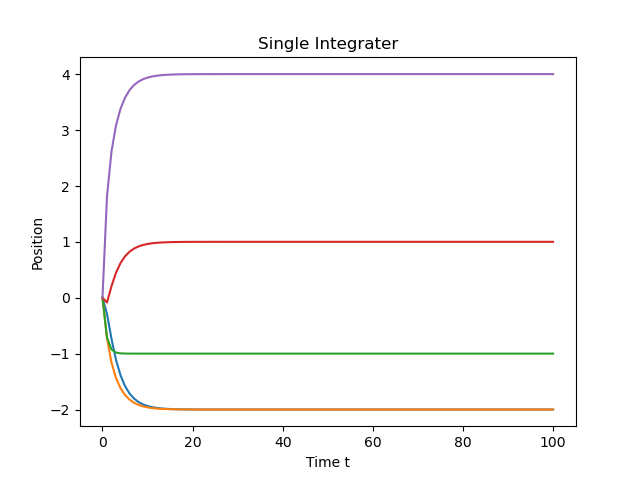
\includegraphics[width=\textwidth]{./img/p5_1.png}
            \caption{Single Integrater}
        \end{subfigure}
        \begin{subfigure}{0.4\textwidth}
            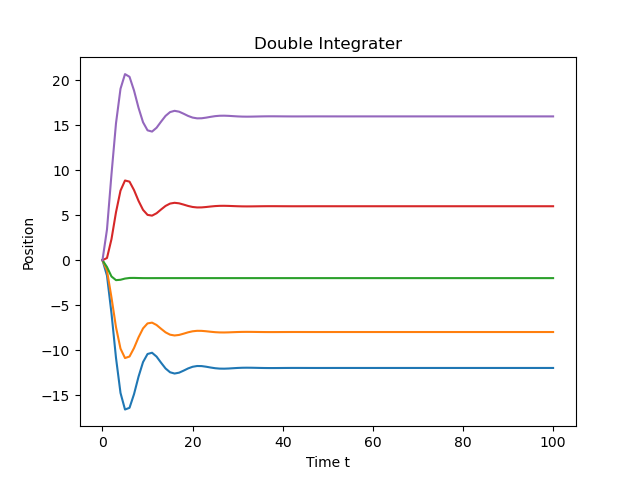
\includegraphics[width=\textwidth]{./img/p5_2.png}
            \caption{Double Integrater position}
        \end{subfigure}
        \begin{subfigure}{0.4\textwidth}
            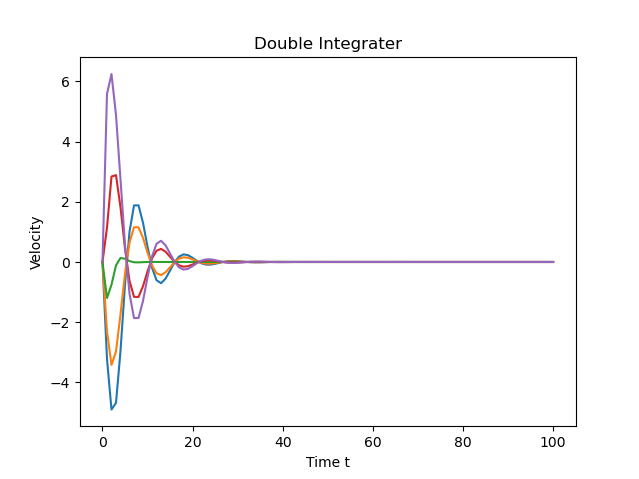
\includegraphics[width=\textwidth]{./img/p5_3.png}
            \caption{Double Integrater velocity}
        \end{subfigure}
        \begin{subfigure}{0.4\textwidth}
            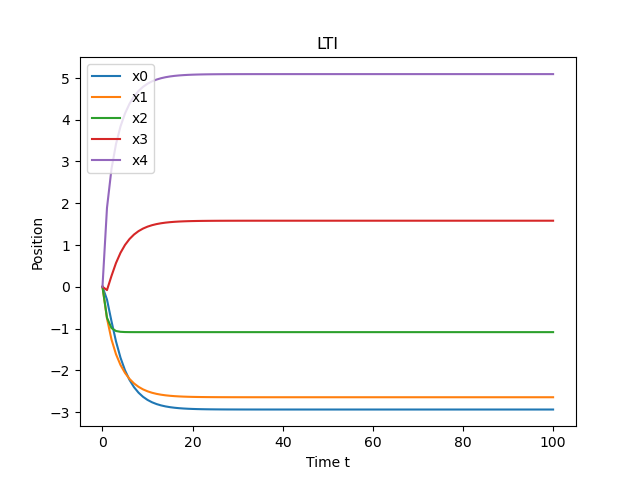
\includegraphics[width=\textwidth]{./img/p5_5.png}
            \caption{LTI stable}
        \end{subfigure}
        \begin{subfigure}{0.4\textwidth}
            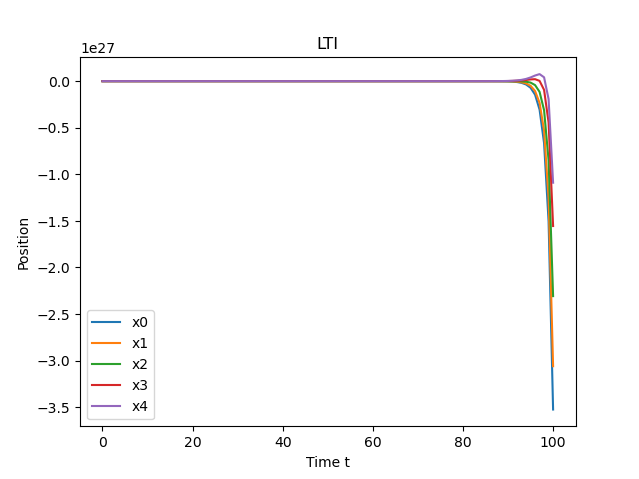
\includegraphics[width=\textwidth]{./img/p5_6.png}
            \caption{LTI Unstable}
        \end{subfigure}
    \end{figure*}
    Since we know that single and double integrater agents achieves desired position and velocity (except for the case when the double integrater has inconsistent desired velocity when desired position is achieved), example for unstable formation is provided only for LTI case. I am going to set all the initial condition to be 0, including velocity.
    For the single integrater agents, I have set the $z_ref = [0, 1,2,3]$, and, for the double integrater agents, $z_ref = [0, 1,2,3]$, and $ \dot z_ref = [4,5,6,7]$. In fact, my velocity profile for double integrater is not consistent with the position, and their velocity profile seems like converged to 0, but it is acutally oscillating if you were to zoom in. For LTI stable agents, $z_ref = [0, 1,2,3]$ were given with $a = 0.1$, $b = 1$, $k = 1$. It is worth potinting out that this LTI model becomes single integrater model, when $a = 0$, and therefore shows similar behavior as single integrater when a is small. However, the LTI model is stable only when $a-\lambda_i(G) k b < 0$, so I used $a = 1$, $b = 1$, $k = 1$ to simulate unstable formation.
\end{problem}
\section*{code for p2 b}
\begin{minted}{python3}
import networkx as nx
import matplotlib.pyplot as plt

def main():
    n = 3
    G = nx.empty_graph(n, create_using=nx.DiGraph)
    G.add_edges_from([(0, 1), (0, 2)])
    pos = nx.spring_layout(G)
    plt.figure()
    nx.draw_networkx_nodes(G, pos, cmap=plt.get_cmap('jet'), node_size = 500)
    nx.draw_networkx_labels(G, pos)
    nx.draw_networkx_edges(G, pos,G.edges(),width=3,  arrows=True)
    G_reverse = nx.reverse(G)
    pos = nx.spring_layout(G_reverse)
    plt.figure()
    nx.draw_networkx_nodes(G_reverse, pos, cmap=plt.get_cmap('jet'), node_size = 500)
    nx.draw_networkx_labels(G_reverse, pos)
    nx.draw_networkx_edges(G_reverse, pos,G_reverse.edges(), width=3, arrows=True)
    plt.show()
if __name__ == "__main__":
    main()
\end{minted}
\section*{code for p2 c}
\begin{minted}{python3}
import networkx as nx
import matplotlib.pyplot as plt

def main():
    n = 5
    G = nx.empty_graph(n, create_using=nx.Graph)
    G.add_edges_from([(1, 0), (1, 2), (3, 2), (3,4)])
    pos = nx.spring_layout(G)
    plt.figure()
    nx.draw_networkx_nodes(G, pos, cmap=plt.get_cmap('jet'), node_size = 500)
    nx.draw_networkx_labels(G, pos)
    nx.draw_networkx_edges(G, pos,G.edges(),width=2,  arrows=True)
    G = nx.empty_graph(n, create_using=nx.DiGraph)
    G.add_edges_from([(1, 0), (1, 2), (3, 2), (3,4)])
    pos = nx.spring_layout(G)
    plt.figure()
    nx.draw_networkx_nodes(G, pos, cmap=plt.get_cmap('jet'), node_size = 500)
    nx.draw_networkx_labels(G, pos)
    nx.draw_networkx_edges(G, pos,G.edges(), width=2, arrows=True)
    G_reverse = nx.reverse(G)
    pos = nx.spring_layout(G_reverse)
    plt.figure()
    nx.draw_networkx_nodes(G_reverse, pos, cmap=plt.get_cmap('jet'), node_size = 500)
    nx.draw_networkx_labels(G_reverse, pos)
    nx.draw_networkx_edges(G_reverse, pos,G_reverse.edges(),width=2,  arrows=True)
    plt.show()
if __name__ == "__main__":
    main()
\end{minted}
\section*{code for p3}
\begin{minted}{python3}
import random
import networkx as nx
import matplotlib.pyplot as plt
import numpy as np
from scipy.integrate import odeint
from mpl_toolkits import mplot3d
def assess_x_1(U, x_0):
    delta_t = np.log(2/3)
    poses = np.matmul(np.exp(-delta_t *nx.laplacian_matrix(U).toarray()),x_0.T)\
    
    print(np.exp(-delta_t *nx.laplacian_matrix(U).toarray()))
    print(poses)
def main():

    n = 5
    G = nx.Graph()
    G.add_node(0)
    H = nx.complete_graph(n-1)
    U = nx.disjoint_union(G, H)
    pos = nx.spring_layout(U)
    U.add_edges_from([(0,1)])
    Delta = 1
    x_0 = np.zeros(n)
    x_0[0] = Delta *2
    x_0[1] = Delta
    
 
    assess_x_1(U, x_0)
    plt.figure()
    nx.draw_networkx_nodes(U, pos, cmap=plt.get_cmap('jet'), node_size = 500)
    nx.draw_networkx_labels(U, pos)
    nx.draw_networkx_edges(U, pos,U.edges(),width=2,  arrows=True)
    plt.show()
if __name__ == "__main__":
    main()



\end{minted}
\section*{code for p4}
\begin{minted}{python3}
import random
import networkx as nx
import matplotlib.pyplot as plt
import numpy as np
from scipy.integrate import odeint
from mpl_toolkits import mplot3d
import math



def show(graph): 
    plt.figure()
    poses = nx.get_node_attributes(graph, 'pos')
    nx.draw_networkx_edges(graph, pos = poses,edgelist=graph.edges(),arrows=True)
    nx.draw_networkx_nodes(graph, pos = poses, nodelist=graph.nodes() ,label=True)
    nx.draw_networkx_labels(graph, pos=poses)
    plt.show()
def random_graphs_init(graph,num):
    poses = {i: (np.random.randint(i+10),np.random.randint(i+10)) for i in range(num)}
    vels = {i: (0,0) for i in range(num)}
    nx.set_node_attributes(graph,poses, "pos")
    nx.set_node_attributes(graph, vels, "vel")
    graph.add_edges_from([(i, i+1) for i in range(len(graph.nodes())-1)])
    graph.add_edges_from([(i+1, i) for i in range(len(graph.nodes())-1)])
    graph.add_edges_from([(num-1, 0), (0, num -1)])

    return graph

def get_formation_ref(num):
    l=[]
    [l.extend([v[0],v[1]]) for k,v in nx.get_node_attributes(D, 'pos').items()]
    x_mean = sum(l[:num])/num
    y_mean = sum(l[num:])/num
    thetas = np.linspace(0, 2*np.pi, num)
def create_z_ref(l, num, int_type):
    #uniformly distributed
    show(D)

    x_mean = sum(l[:num])/num
    y_mean = sum(l[num:])/num
    thetas = np.linspace(0, 2*np.pi, num)
    match int_type:
        case 1:
             z_ref = np.linspace(1, 2*num, 2*num)
             print(z_ref)
        case 2:
             z_ref = [1,1,1,1,0,0,0,0]
        case _:
             z_ref = np.linspace(0, num-1, num)
    return z_ref

def single_xdot(x, t, D, z_ref,k):

    # L_D_bar = nx.laplacian_matrix(D.to_undirected(reciprocal=False, as_view=False)).toarray()
    # D_D = nx.incidence_matrix(D, oriented=True).toarray()
    # return -k *np.matmul(L_D_bar, x) + k * np.matmul(D_D,z_ref)
    poses = {i: (x[i],x[i+num]) for i in range(num)}
    vels = {i: (0,0) for i in range(num)}
    nx.set_node_attributes(D,poses, "pos")
    nx.set_node_attributes(D, vels, "vel")
    return -(x-z_ref)

num = 5
D =nx.empty_graph(num,create_using=nx.DiGraph())
# D = nx.gnm_random_graph(num, (num -1)*(num-2)/2, directed=True)
D = random_graphs_init(D,num)
z_ref = []
def main():
    
    k = 1
    
    labels = []
    for i in range(num):
        labels.append(f"x{i}")
    
    t = np.linspace(0, 10, 101)
    l=[]
    [l.extend([v[0],v[1]]) for k,v in nx.get_node_attributes(D, 'pos').items()]
    print(f"input for odeint: {l}")
    ## Single
    z_ref = create_z_ref(l,len(D.nodes()),1)
    # np.append(list(nx.get_node_attributes(D, 'pos_x')),list(nx.get_node_attributes(D, 'pos_y')))
    
    trajectory_y = odeint(single_xdot,l, t, args=(D, z_ref, k))
    plt.figure()
    plt.plot(t, trajectory_y[:,:num], label = labels)
    plt.xlabel("Time t")
    plt.ylabel("Position")
    plt.title("Double Integrater")
    plt.figure()
    plt.plot(t, trajectory_y[:,num:], label = labels)
    plt.xlabel("Time t")
    plt.ylabel("Velocity")
    # plt.title("Double Integrater")
    plt.figure()
    plt.plot( trajectory_y[:,num:],trajectory_y[:,:num], label = labels)
    plt.plot(z_ref[num:], z_ref[:num])
    # plt.xlabel("Time t")
    # plt.ylabel("Velocity")
    # plt.title("Double Integrater")
    show(D)
    plt.show()
if __name__ == "__main__":
    main()
\end{minted}
\section*{code for p5}
\begin{minted}{python3}
import random
import networkx as nx
import matplotlib.pyplot as plt
import numpy as np
from scipy.integrate import odeint
from mpl_toolkits import mplot3d
def random_graphs_init(graph,num):
    poses = 0
    vels = 1
    nx.set_node_attributes(graph,poses, "pos")
    nx.set_node_attributes(graph, vels, "vel")
    # poses.append(0)
    graph.add_edges_from([(i, i+1) for i in range(len(graph.nodes())-1)])

    edges = {(i, i+1):{graph.nodes[i+1]['pos'] - graph.nodes[i]['pos']}  for i in range(len(graph.nodes())-1) }
    nx.set_edge_attributes(graph, edges, "edge_length")
    return graph

def create_z_ref(num, int_type):
    #uniformly distributed
    
    match int_type:
        case 1:
                z_ref = np.linspace(0, num-1, num)
        case 2:
                z_ref = [1,1,1,1,0,0,0,0]
        case _:
                z_ref = np.linspace(0, num-1, num)
    return z_ref

def single_xdot(x, t, D, z_ref,k):

    L_D_bar = nx.laplacian_matrix(D.to_undirected(reciprocal=False, as_view=False)).toarray()
    D_D = nx.incidence_matrix(D, oriented=True).toarray()
    return -k *np.matmul(L_D_bar, x) + k * np.matmul(D_D,z_ref)

def double_xdot(x, t, D, z_ref,k):
    k = 0.1
    L_D_bar = nx.laplacian_matrix(D.to_undirected(reciprocal=False, as_view=False)).toarray()
    D_D = k*nx.incidence_matrix(D, oriented=True).toarray()
    
    L_D_bar = -k *np.kron([[0,0], [1,1]] ,L_D_bar) + np.kron([[0,1], [0,0]], np.eye(len(x)//2))
    
    
    D_D = k*np.kron([[0,0], [1,1]] ,D_D) 
    
    return np.matmul(L_D_bar, x) + np.matmul(D_D,z_ref)

def LTI_xdot(x, t, D, z_ref,k):
    a = .1
    b = 1
    z_t = np.matmul(nx.incidence_matrix(D, oriented=True).toarray().T, x)
    u = k*np.matmul(nx.incidence_matrix(D, oriented=True).toarray(), (z_ref - z_t)) 
    return a*x + b*u
def main():
    nums = [5]
    k = 1
    
    for num in nums:
        labels = []
        for i in range(num):
            labels.append(f"x{i}")
        D =nx.empty_graph(num,create_using=nx.DiGraph())
        # D = nx.gnm_random_graph(num, (num -1)*(num-2)/2, directed=True)
        D = random_graphs_init(D,num)
        # z_ref = create_z_ref(len(D.edges()),1)
        t = np.linspace(0, 30, 101)
        
        # trajectory_x = odeint(single_xdot, list(nx.get_node_attributes(D, "pos").values()), t, args=(D, z_ref, k))
        # plt.figure()
        # plt.plot(t, trajectory_x, label = labels)
        # plt.xlabel("Time t")
        # plt.ylabel("Position")
        # plt.title("Single Integrater")
        z_ref = create_z_ref(len(D.edges()),2)
        print(z_ref)
        pos_vel = []
        for i in range(len(D.nodes())):
            pos_vel.append(nx.get_node_attributes(D, "pos")[i])
            pos_vel.append(nx.get_node_attributes(D, "vel")[i])
        # pos_vel = np.append(list(nx.get_node_attributes(D, "pos").values()), list(nx.get_node_attributes(D, "vel").values()))
        # trajectory_double = odeint(double_xdot, pos_vel , t, args=(D, z_ref, k))
        # plt.figure()
        # plt.plot(t, trajectory_double[:,:num], label = labels)
        # plt.xlabel("Time t")
        # plt.ylabel("Position")
        # plt.title("Double Integrater")
        # plt.figure()
        # plt.plot(t, trajectory_double[:,num:], label = labels)
        # plt.xlabel("Time t")
        # plt.ylabel("Velocity")
        # plt.title("Double Integrater")
        z_ref = create_z_ref(len(D.edges()),3)
        trajectory_LTI = odeint(LTI_xdot, list(nx.get_node_attributes(D, "pos").values()) , t, args=(D, z_ref, k))
        plt.figure()
        plt.plot(t, trajectory_LTI, label = labels)
        plt.xlabel("Time t")
        plt.ylabel("Position")
        plt.title("LTI")
    plt.legend()
    plt.show()

if __name__ == "__main__":
    main()
\end{minted}
\end{document}